\documentclass[11pt,]{article}
\usepackage{lmodern}
\usepackage{amssymb,amsmath}
\usepackage{ifxetex,ifluatex}
\usepackage{fixltx2e} % provides \textsubscript
\ifnum 0\ifxetex 1\fi\ifluatex 1\fi=0 % if pdftex
  \usepackage[T1]{fontenc}
  \usepackage[utf8]{inputenc}
\else % if luatex or xelatex
  \ifxetex
    \usepackage{mathspec}
    \usepackage{xltxtra,xunicode}
  \else
    \usepackage{fontspec}
  \fi
  \defaultfontfeatures{Mapping=tex-text,Scale=MatchLowercase}
  \newcommand{\euro}{€}
\fi
% use upquote if available, for straight quotes in verbatim environments
\IfFileExists{upquote.sty}{\usepackage{upquote}}{}
% use microtype if available
\IfFileExists{microtype.sty}{%
\usepackage{microtype}
\UseMicrotypeSet[protrusion]{basicmath} % disable protrusion for tt fonts
}{}
\usepackage[margin=2cm]{geometry}
\usepackage{graphicx}
\makeatletter
\def\maxwidth{\ifdim\Gin@nat@width>\linewidth\linewidth\else\Gin@nat@width\fi}
\def\maxheight{\ifdim\Gin@nat@height>\textheight\textheight\else\Gin@nat@height\fi}
\makeatother
% Scale images if necessary, so that they will not overflow the page
% margins by default, and it is still possible to overwrite the defaults
% using explicit options in \includegraphics[width, height, ...]{}
\setkeys{Gin}{width=\maxwidth,height=\maxheight,keepaspectratio}
\ifxetex
  \usepackage[setpagesize=false, % page size defined by xetex
              unicode=false, % unicode breaks when used with xetex
              xetex]{hyperref}
\else
  \usepackage[unicode=true]{hyperref}
\fi
\hypersetup{breaklinks=true,
            bookmarks=true,
            pdfauthor={Fred Boehm, Statistics 998},
            pdftitle={Identifying myocardial infarction risk factors in the Wisconsin Longitudinal Study to aid in intervention program design},
            colorlinks=true,
            citecolor=blue,
            urlcolor=blue,
            linkcolor=magenta,
            pdfborder={0 0 0}}
\urlstyle{same}  % don't use monospace font for urls
\setlength{\parindent}{0pt}
\setlength{\parskip}{6pt plus 2pt minus 1pt}
\setlength{\emergencystretch}{3em}  % prevent overfull lines
\setcounter{secnumdepth}{0}

%%% Use protect on footnotes to avoid problems with footnotes in titles
\let\rmarkdownfootnote\footnote%
\def\footnote{\protect\rmarkdownfootnote}

%%% Change title format to be more compact
\usepackage{titling}
\setlength{\droptitle}{-2em}
  \title{Identifying myocardial infarction risk factors in the Wisconsin
Longitudinal Survey to aid in intervention program design}
  \pretitle{\vspace{\droptitle}\centering\huge}
  \posttitle{\par}
  \author{Fred Boehm, Statistics 998}
  \preauthor{\centering\large\emph}
  \postauthor{\par}
  \predate{\centering\large\emph}
  \postdate{\par}
  \date{March 31, 2015}


\usepackage[hypcap]{caption}
\usepackage{subcaption}
\usepackage[colorinlistoftodos=true]{todonotes}
\usepackage{dcolumn}
\usepackage{booktabs}


\begin{document}

\maketitle


\listoftodos

\subsection{Abstract}\label{abstract}

\subsection{Introduction}\label{introduction}

Coronary artery disease (CAD) is a leading cause of death in the United
States and much of North America and Europe. In 2011, one American died
of CAD every 40 seconds, on average, and 155,000 of those deaths were
people aged less than 65 years.\footnote{Mozaffarian et al., ``Executive
  Summary.'' } One manifestation of CAD is a myocardial infarction (MI),
which is also called a ``heart attack''. A MI results from a clot in a
coronary artery that diminishes blood flow to the heart muscle, or
myocardium. If blood flow disruption persists for a sufficiently long
time, the muscle may die, or infarct. The irreparable dead heart muscle
diminishes the overall ability of the heart to pump blood. Severe MIs
may lead to a patient's death.

Epidemiologists have identified modifiable and non-modifiable risk
factors that contribute to CAD risk. Smoking is among the strongest
modifiable risk factors, and is thought to elevate CAD risk by
triggering elevations in inflammatory molecules in the bloodstream.
\_\_\_\_
\todo[inline, color = red]{What is mechanism for smoking causing CAD?}.
Diabetes mellitus and hypertension (systolic or diastolic) are typically
considered non-modifiable risk factors, although their contribution to
CAD risk may be reduced in patients who undertake dramatic lifestyle
interventions, such as exercise programs and diet with weight loss.
Non-modifiable risk factors include age, a family history of CAD and
presence of certain genetic variants
\todo[inline, color = pink]{what are other known risk factors?}.

Our collaborators at the Wisconsin Longitudinal Study (WLS) have
undertaken an investigation on a subset of WLS participants with the
goal of identifying CAD risk factors in the WLS study population. The
ultimate goal of this project is to develop an intervention program to
reduce CAD morbidity and mortality in Wisconsin. The investigators would
like to extend such an intervention program to Wisconsin residents who
are not WLS subjects. Our goal in this report is to identify risk
factors for MI among WLS participants.

\subsection{Study design}\label{study-design}

The Wisconsin Longitudinal Study (WLS) is a long-term study of a random
sample of 10,317 men and women who graduated from Wisconsin high schools
in 1957. According to the WLS website ``WLS provides an opportunity to
study the life course, intergenerational transfers and relationships,
family functioning, physical and mental health and well-being, and
morbidity and mortality from late adolescence through 2011.''\footnote{``Wisconsin
  Longitudinal Study''. }

\todo[inline, color = blue]{need more info on WLS?}

Our collaborators collected data from the original respondents or their
parents in 1957, 1964, 1975, 1992, 2004, and 2011; from a selected
sibling in 1977, 1994, 2005, and 2011; from the spouse of the original
respondent in 2004; from the spouse of the selected sibling in 2006; and
from widow(er)s of the graduates and siblings in 2006.

\subsection{Data description}\label{data-description}

Our collaborators shared with us a data set that contains records for
19095 individuals (including original subjects and siblings) with 310
variables per subject. 9363 subjects responded (with yes or no) to the
2011 question of whether they had ever had a heart attack.

\subsection{Exploratory data analyses}\label{exploratory-data-analyses}

Since our WLS data included 310 variables, we won't provide summaries
for all of them in this document. Instead, we focus our exploratory
analyses on our response variables (HAC2011, HAC2004, HACinc, doc2011,
doc2004, docinc) and covariates that other researchers have identified
as associated with coronary artery disease.

Age is known, from epidemiologic studies, to be a strong risk factor for
CAD, with older individuals having an elevated CAD risk.

\todo[inline, color = green]{what to explore for categorical data? Only the proportion in each category????}

\subsection{Statistical modeling}\label{statistical-modeling}

We used statistical modeling to try to identify covariates that
associated with six distinct outcomes: 1) HAC2004, 2) HAC2011, 3)
DOC2004, 4) DOC2011, 5) new self-reported heart attacks (from 2004 to
2011) and 6) new heart attack per doctor's report (from 2004 to 2011).
For a subject to qualify as a ``new'' self-reported heart attack, they
must have responded ``No'' in 2004 and ``Yes'' in 2011. Analogous
definition applies for ``new'' doctor-reported heart attack.

We found that HAC2004 had 11534 non-missing responders (with 665
responding ``Yes'' and 10869 responding ``No''). Counts for other
variables are provided in Appendix A.

\subsubsection{Statistical modeling with Framingham study
predictors}\label{statistical-modeling-with-framingham-study-predictors}


\begin{table}
\begin{tabular}{l r}

Framingham study variable & WLS Variable\\
\hline
Sex & Sex\\
Quantitative total cholesterol & highchol2011, highchol2004\\
Quantitative HDL cholesterol & None\\
Smoking & smokever2011 (Columns 61 to 87 aim to quantify smoking) \\
Diabetes & diabetes2004, diabetes2011\\
Age & Age\\
Systolic BP & highbp2004, highbp2011* \\
Treated for high blood pressure & None\\
\hline
\end{tabular}
\caption{Framingham study variables and their closest analogs in WLS. (* SBP not available, so we used reported "high BP".)}
\label{table:fram2wls} % need label after the caption{} line
\end{table}

We identified those variables in the WLS that closely match those in the
Framingham study\footnote{D'Agostino et al., ``General Cardiovascular
  Risk Profile for Use in Primary Care the Framingham Heart Study.'' } (
Table \ref{table:fram2wls}). It's important to note that the Framingham
study used survival analysis methods, including Cox proportional hazards
regression, to identify risk factors for a cardiovascular event. Thus,
their study design, analysis, and purpose differ from ours.

Because the risk factors from the Framingham study have strong effect
sizes, are easily interpreted, and widely used by both physicians and
public health scientists, we decided to perform logistic regression
analyses with solely those WLS variables that most closely matched the
Framingham variables. We analyzed each of the 6 outcomes of interest.
For each outcome variable, we fitted a logistic regression model using
the entire data set (omitting those subjects with missing data). We then
transformed the fitted logit values to probabilities before plotting a
receiver operating characteristic (ROC) curve for each model, in which
we use the fitted probabilities to examine the trade-off between
specificity and sensitivity. We also calculated the area under the curve
(AUC) for each ROC curve.\footnote{Robin et al., ``PROC.'' }

\begin{figure}[htbp]
\centering
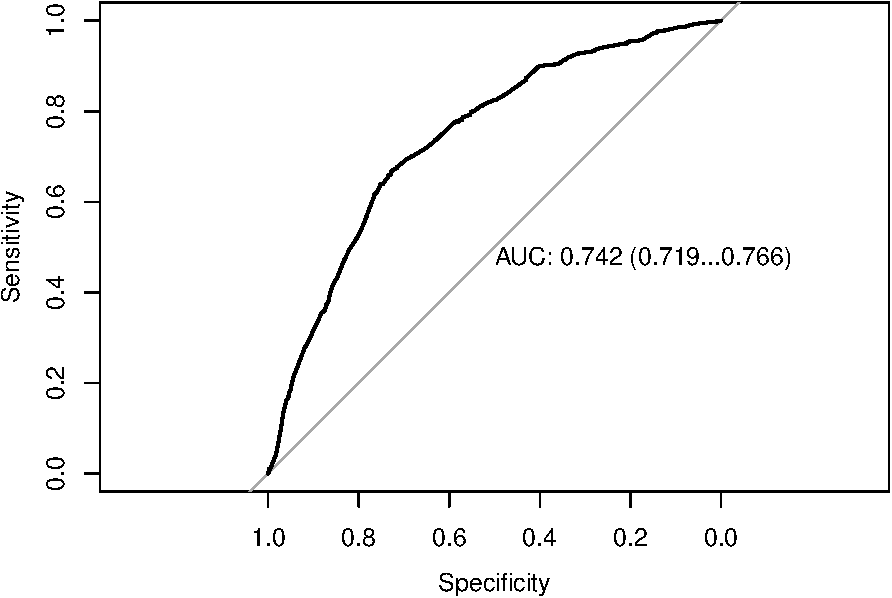
\includegraphics{report2_files/figure-latex/plot-hac2011-1.pdf}
\caption{Receiver operating characteristic curve for the logistic
regression model with outcome HAC2011 and the six Framingham
covariates.}
\end{figure}

\subsubsection{Subgroup-specific
modeling}\label{subgroup-specific-modeling}

\subsection{Results}\label{results}

\todo[inline, color = purple]{Show a single ROC plot \& explain what is meant by "AUC"}

\subsubsection{Comparing statistical models with cross-validation and
area under the curve (AUC)
statistic}\label{comparing-statistical-models-with-cross-validation-and-area-under-the-curve-auc-statistic}

In evaluating our statistical models, we used ``area under the curve''
(AUC) from our receiver operating characteristic (ROC) curves. Each
statistical model was evaluated with 5-fold cross-validation. For those
unfamiliar with cross-validation, five-fold cross-validation means that
we partition the subjects into 5 non-overlapping ``folds'' of
approximately equal size. We then fit 5 models, using 4 of the 5 folds
as the ``training'' set for each fit. For each fit, we then test the
model with fold that wasn't used in the corresponding training set. For
example, for five-fold CV, we first omit fold \#1 and fit the model
using folds 2,3,4, and 5 together. We then test the model using fold
\#1. We then fit a model with folds 1,3,4, and 5 together and test it
with fold \#2. We continue this procedure until all five possible models
are fitted. For each of the five models, we created a received operating
characteristic (ROC) curve and evaluated the area under the curve using
the pROC R package.\footnote{Ibid. }

A ROC curve is a plot of sensitivity against specificity. We created the
ROC curve by varying the threshold cut point for our classifier and
seeing how distinct cut points impact our specificity and sensitivity as
measured on the test set.

\subsection{Discussion}\label{discussion}

\subsection{Future directions}\label{future-directions}

We would like to investigate other tree-based methods, including those
developed by Wei-Yin Loh's research team. The absence of R
implementations of Loh's algorithms prevented us from including them in
our current analysis. We have begun the process of writing code to
implement Loh's algorithms in R, but they are not yet ready for use.

\todo[inline]{explain why we want Loh's algorithms. Might mention why they could be useful in this project.}

A major reason for using Loh's algorithms, such as GUIDE, is their
unbiasedness.\footnote{Loh, ``Classification and Regression Trees.'' }
CART, the algorithm that's implemented in the rpart package, has an
intrinsic selection bias that favors selection of categorical variables
with more discrete values. GUIDE, on the other hand, avoids this
selection bias. In the current scenario, because most of our variables
are either continuous or binary, we're not selection bias is likely to
be a major problem, but we'd still like to compare GUIDE results with
those of CART.

Given the relatively low cost of acquiring genomics data, one possible
future direction is to acquire genomics data for a subset of study
subjects. For example, SNP genotype data from each subject may enable us
to further discriminate those subjects that are at high risk for a CAD
event. In some cases, we may be able to use cheek swabs as sources of
DNA, which would enable data collection by mail. Such knowledge of
genetic risk factors, when coupled with non-genetic risk factors, may be
translated into the proposed intervention program, for example, by
promoting healthy diet and physical activity among those at greatest
risk.

\newpage

\subsection{Appendix A: Supplementary
materials}\label{appendix-a-supplementary-materials}

\newpage 

\subsection{Appendix B: Questions for
client}\label{appendix-b-questions-for-client}

\begin{enumerate}
\def\labelenumi{\arabic{enumi}.}
\item
  What do you intend to do with results from this study?
\item
  How important is prediction of future MI to your scientific goals?
  There may be a tradeoff between prediction and the ability to quantify
  variable effects (for example does smoking increase or decrease risk?
  By how much? Does the effect vary across population subgroups?).
\item
  Why are there so many missing values (NA) for the HA2011 \& HA2004
  variables? Did these subjects not respond to that question? Did they
  respond to the survey at all?
\item
  Which variables do you think are the most meaningful?
\item
  Is incidence of MI between 2004 and 2011 a meaningful outcome? We
  could try to ascertain who had a MI during that interval (from among
  the people who had no MI history in 2004)
\item
  We're considering focusing on established risk factors such as those
  that the Framingham study identified. Is this reasonable? Or do you
  want to try to identify novel risk factors?
\item
  Are the ``created'' variables HAC2011 and HAC2004 better than the
  unadjusted versions? Is there any reason to do separate analyses for
  2011 and 2004? Could we just code ``yes'' for a yes in any year,
  otherwise use 2011 value.\\Why do some responses switch from ``yes''
  in 2004 to ``no'' in 2011---is this because the question specifically
  refers to heart attacks or diagnoses within the last 20 years?
\item
  Should any conditions be excluded as covariates because they can occur
  concurrently with heart disease (e.g.~diabetes, stroke, high blood
  pressure, high cholesterol)? In other words, is there more interest in
  leading indicators?
\item
  Is there interest in separating the effects of covariates gathered in
  multiple years (e.g.~highchol2004, highchol2011)? Should these be
  combined into a single measure? Should 2011 effect be excluded when
  modeling a 2004 response?
\item
  I noticed some ordinal variables (e.g.~education level) are coded as
  integers. Is this consistent for all ordinal variables? Are there any
  non-ordinal categorical variables coded as integers?
\end{enumerate}

\newpage

\subsection{Appendix C: Computing code}\label{appendix-c-computing-code}

\newpage

\subsection{Appendix D: Additional
note}\label{appendix-d-additional-note}

Throughout this report, we tried to adhere to the style suggested by
Leek.\footnote{\emph{The Elements of Data Analytic Style}.} We used the
R statistical environment for all calculations\footnote{R Core Team,
  \emph{R}. }. Mike Wurm performed the tree-based analysis, and the code
for that part is nearly identical to his. The R packages gbm,\footnote{Others,
  \emph{Gbm}. } pROC\footnote{Robin et al., ``PROC.'' } and
rpart\footnote{Therneau, Atkinson, and Ripley, \emph{Rpart}. } played
central roles in our analyses.

\subsection*{References}\label{references}
\addcontentsline{toc}{subsection}{References}

D'Agostino, Ralph B, Ramachandran S Vasan, Michael J Pencina, Philip A
Wolf, Mark Cobain, Joseph M Massaro, and William B Kannel. ``General
Cardiovascular Risk Profile for Use in Primary Care the Framingham Heart
Study.'' \emph{Circulation} 117, no. 6 (2008): 743--53.

Leek, Jeff. \emph{The Elements of Data Analytic Style}. Leanpub,
2015Available at \url{https://leanpub.com/datastyle}.

Loh, Wei-Yin. ``Classification and Regression Trees.'' \emph{Wiley
Interdisciplinary Reviews: Data Mining and Knowledge Discovery} 1, no. 1
(2011): 14--23.

Mozaffarian, Dariush, Emelia J Benjamin, Alan S Go, Donna K Arnett,
Michael J Blaha, Mary Cushman, Sarah de Ferranti, et al. ``Executive
Summary: Heart Disease and Stroke Statistics---2015 Update a Report from
the American Heart Association.'' \emph{Circulation} 131, no. 4 (2015):
434--41.

others, Greg Ridgeway with contributions from. \emph{Gbm: Generalized
Boosted Regression Models}, 2015.
\url{http://CRAN.R-project.org/package=gbm}R package version 2.1.1.

R Core Team. \emph{R: A Language and Environment for Statistical
Computing}. Vienna, Austria: R Foundation for Statistical Computing,
2015. \url{http://www.R-project.org/}.

Robin, Xavier, Natacha Turck, Alexandre Hainard, Natalia Tiberti,
Frédérique Lisacek, Jean-Charles Sanchez, and Markus Müller. ``PROC: An
Open-Source Package for R and S+ to Analyze and Compare ROC Curves.''
\emph{BMC Bioinformatics} 12 (2011): 77.

Therneau, Terry, Beth Atkinson, and Brian Ripley. \emph{Rpart: Recursive
Partitioning and Regression Trees}, 2015.
\url{http://CRAN.R-project.org/package=rpart}R package version 4.1-9.

``Wisconsin Longitudinal Study''.
\url{http://www.ssc.wisc.edu/wlsresearch/}, 2015Accessed on
21-March-2015.

\end{document}
